\section{Community Split? Evidences of User Registration, Posting Behavior and Reputation Score}
%In this part, we mainly analyse whether it is necessary to build multilingual Stack Overflow by deeply compare the user activity, the knowledge base status and the areas of focus between Stack Overflow main site and Russian Stack Overflow site. The combination of all research results can lead to a solid conclusion for the meaning of multilingual Q\&A community development. \par 

\begin{comment}
For instance, Table~\ref{tab:multiSO} not only shows the number of posts, comments, users, but also the overlap users between each new site with the main site.
The high percentage of the overlap of users may negatively influence the main site, but is needs further quantitative analysis to be confirmed.

%\begin{table}[h!]
\begin{table}
	\centering
	\caption{Statistics of Stack Overflow main site and its lingual variants (By 8th Dec. 2017)}
	\label{tab:multiSO}
	\begin{tabular}{lrrrr}
		Site & \#User & \#Both Sites User & \#Post & \#Comment\\
		\hline
		Main site & 8,123,937 & * & 38,485,047 & 62,389,331\\
		Russian & 98,125 & 51,415(52.4\%) & 400,185 & 750,143\\
		Portuguese & 70,985 & 42,455(59.8\%) & 202,002& 361,108\\
		Spanish & 60,110 & 34,833(57.9\%) & 94,827 & 155,098\\
		Japanese & 14,777 & 7,818(52.9\%) & 30,571& 29,395\\
	\end{tabular}
\end{table}	
\end{comment}

Users, especially the core users are crucial to the success of Q\&A sites~\cite{mamykina2011design}, as they play an important role in asking and answering questions, and in curating post content and quality.
Will the multi-lingual sites result in the split of user community by the languages?
What kinds of users contribute the most to the multi-lingual sites?
Will multi-lingual sites affect the posting behavior of users who have accounts in both English and non-English sites?
We answer these questions by analyzing user registration, user reputation score, and user posting behavior.
%Some users have accounts in both Stack Overflow and Russian Stack Overflow.


\subsection{User Registration}
%\textcolor{red}{CCY: We tune-down the \textbf{migration} and avoid mentioning it in the paper.}
%Focusing on this intersection user base, the user migration can be measured by comparing their account creation dates of both site. 

By December 8th, 2017, there are 8,123,937 users in the English Stack Overflow (ESO) site and 98,125 users in the Russian Stack Overflow (RSO) site. 
As both sites belong to Stack Exchange networks~\cite{web:StackExchange}, we can identify the intersection of users who own both ESO and RSO accounts by their Stack Exchange ID.
We find that 51,415 users own both accounts at the same time, accounting for 52.4\% of the total number of the users in Russian Stack Overflow.

We further check the account registration time of these 51,415 users.
Among these 51,415 users, 32,288 (62.8\%) sign up their ESO account first and then sign up RSO account.
Those users account for 32.9\% of the 98,125 registered users in RSO which shows the importance of the ESO site to the development of the RSO site.
However, compared with the total 8.1 million users in ESO, 32,288 users account for only 0.4\%.
Therefore, even all of these 32,288 users stop using ESO and contribute only to RSO, it will not result in a significant loss for ESO.
Let alone many uses who own both accounts do not stop contributing to ESO after signing up RSO (see Section~\ref{sec:userpostingbehavior}). 
On the other hand, 19,125 (37.2\%) users sign up their RSO account first, and then sign up ESO account.
It means that to some extent, the launch of RSO may help to attract users to ESO.
This could further reduce the potential loss of users in the English site.

 
\begin{comment}
\begin{figure}[!h]
	\centering
	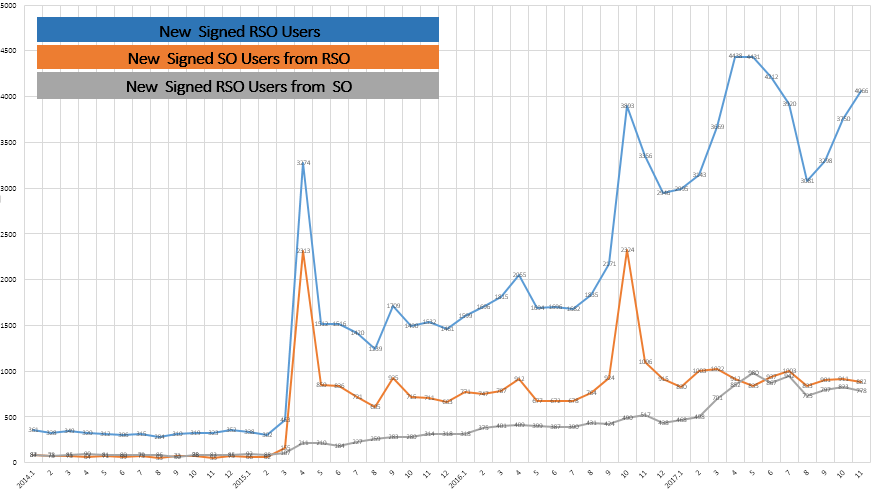
\includegraphics[width = 0.7\textwidth]{figures/userflow.png}
	\caption{The Sign Up for different sites}
	\centering
	\text{\scriptsize(SO for Stackoverflow and RSO for Russian Stackoverflow)}
	\label{fig:signup}
\end{figure} 
 
To illustrate the user migration in details, Figure~\ref{fig:signup} presents the statics of the users who sign up a Russian Stack Overflow account from Jan 1st, 2014 (the launch time of Russian Stack Overflow) to Dec. 8th, 2017. 
As shown in the figure, the new users who migrated from Stack Overflow main site 
occupy a high proportion, and also the Russian site attracts and \textcolor{red}{feedbacks a growing 
number of users ??what does this mean? not good English} to the main site with the time going by. 
In other words, the main 
site and the multilingual version both have a positive effect on the other one, which 
means both of them can \textcolor{red}{assist the development of the other ??this conclusion contradicts to that of last paragraph!}. This phenomenon means 
the development of multilingual version is helpful for the development of the main 
site.
%This phenomenon means the development of multilingual version is helpful for the development of the main site.	
\end{comment}

%\subsection {User Location}

Next, we would like to investigate the impact of building RSO site to the specific group of users in the original ESO site who can speak Russian.
To that end, we try to identify users in ESO who are from Russia or can speak Russian.
In Stack Overflow, users can create their own profiles by filling in their names, location, AboutMe (self introduction), GitHub link, etc.
Fig.~\ref{fig:userportfolio} shows an example user profile who can speak Russian.
We first check if the user's location is in Russia.
If the location contains any Russian letters, we regard the place as in the Russia.
If the location is written in English, we determine whether the location is in Russia by checking the Russian cities list on Encyclopaedia Britannica\footnote{\url{https://www.britannica.com/topic/list-of-cities-in-Russia-2040243}}.
We assume that the users whose location is in Russia can speak Russian.
%Through the location, we find \textcolor{red}{??} users who may be from Russia.
Then for other users who do not have location information, we further check if their AboutMe contains any Russian letters, and if so we also regard such users as ones who can speak Russian.

\begin{figure}
	\centering
	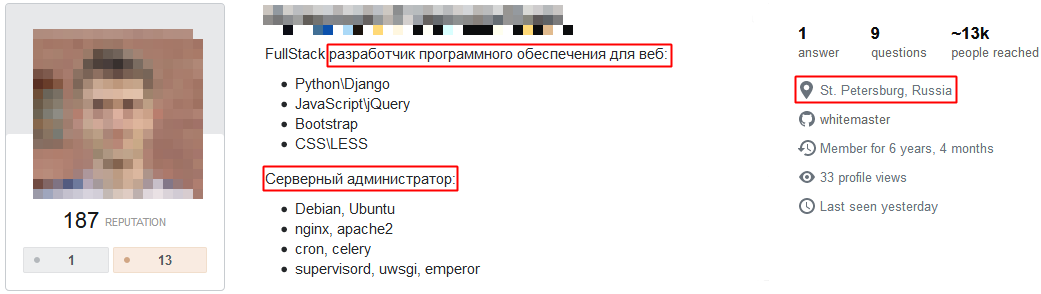
\includegraphics[width = 0.8\textwidth]{figures/userportfolio.png}
	\caption{One user portfolio in English Stack Overflow. This user may speak Russian.}
	\centering
	\label{fig:userportfolio}
\end{figure}

Using the above two heuristics, we find in total 34,705 users in ESO who may speak Russian.
Among these users, 10,699 (30.8\%) have registered RSO.
Within these 10,699 users, 6,537 (61.1\%) users sign up ESO first, and the rest 4,162 (38.9\%) users sign up RSO first.
While for the other users in ESO (8,089,232), only 40,716 (0.5\%) have RSO accounts.
The results show that, compared with users who do not speak Russian, RSO does attract many potentially Russian-speaking users in ESO. 
However, this does not mean a unidirectional loss of users from ESO to RSO, because RSO also helps attract users to ESO.
  
%It indicates that not only can Russian Stack Overflow attract users in Stack Overflow, but Stack Overflow can also benefit from Russian Stack Overflow.
%Such phenomenon mitigates the user loss of Stack Overflow.

\begin{comment}
To identity the Russian users on the Stack Overflow main site, the location information of registered users has also been analyzed. The users whose location are places in Russia (either written in English or in Russian) as well as the ones whose AboutMe sections contain Russians are marked as Russian related users, indicating their native language is probably Russian. The collected statistics is shown in Table~\ref{tab:loc}. Under this assumption, there are \textcolor{red}{34,705 Russian related users ??why not 51415 in Section 2.1.1?} registered on the Stack Overflow main site. Among these users, 10,699 (30.8\%) users have the Russian Stack Overflow account at the same time which means the rest majority of Russian users only use the main site. 
Also, within these 10,699 users, 6,537 (61.1\%) users migrated from main site to Russian site and 4,162 (38.9\%) users migrated from Russian site to main site. Most Russian related users (69.2\%) on the Stack Overflow still only have the main site account rather than migrating to the Russian Stack Overflow. 
 
\begin{table}[h!]
	\centering
	\caption{Location and AboutMe information analysis (users count among 8,123,937 main site users)}
	\label{tab:tablex}
	\begin{tabular}{lrr}
		Filter & \#Location Info. & \#AboutMe Info.\\
		\hline
		contain non-englsih word & 111,006  &  35,000\\
		contain Russian Letter & 9,858 &  2,079\\
		contain Russian Places & 24,468 & 1,718\\
	\end{tabular}
    \begin{tabular}{lr}
    	\hline
    	Total Russian related users: & 34,705\\
    	Russian related users with RSO account: & 10,699\\
    \end{tabular}
	\label{tab:loc}
\end{table}	
\end{comment}
 
\subsection{User Posting Behavior}
\label{sec:userpostingbehavior}

In a Q\&A website, the main user interaction is to ask and answer questions.
We regard both questions and answers as posts.
In RSO, there are 400,185 posts as of December 8th, 2017.
We count the number of posts created by different users.
The results can be seen in Table~\ref{tab:postnumber}.
We can see that 6,201 (6.3\%) users who have created more than 10 posts have contributed to 75.9\% posts in RSO.
So, we regard these 6,201 users as the core users in RSO.

\begin{table}
	\centering
	\small
	\caption{Statics of user posting behavior in Russian Stack Overflow}
	\label{tab:postnumber}
	\begin{tabular}{lllll}
		\hline
		\textbf{\#Post by User} & \textbf{\#Post} & \textbf{\% of All Posts} & \textbf{\#User} & \textbf{\% of All Users} \\
		\hline
		$>=$2 &372,046&92.9\%&24,908&25.4\%\\
		$>=$4 &345,543&86.3\%&13,526&13.8\%\\
		$>=$6 &328,398&82.1\%&9,644&9.8\%\\
		$>=$8 &314,833&78.7\%&7,537&7.7\%\\
		$>=$10&303,604&75.9\%&6,201&6.3\%\\
		\hline
	\end{tabular}
\end{table}	

\begin{comment}
Post is the prime part in the content of a Q\&A websites since post is the rising of the question as well as the origin of the answers and comment. It is also a very suitable variable to find the active users and popular topics in the Q\&A website community. Although every user has the right to post a question and add comments, the composition of the knowledge base ought to obey \textcolor{red}{the Pareto Law, which means 20\% of the users make 80\% of the contribution ??where do you find this? any reference or support? in general, literature says power law. how can know 20\% versus 80\%?}.

Imagine that a post is a single unit, and millions of posts consist of the knowledge base, and each post includes maybe a lot of answers and comments in the tree structure. 
From Table 1 it is already clear that there are totally 400,185 posts for the Russian Stack Overflow, and using the unique account id to calculate the amount of post for each user on Russian Stack Overflow, the results are presented in Table~\ref{tab:postnumber}. 	

From the table, the static distribution can be easily seen. As mentioned above, with the number of a single user post sum growing, the user proportion decrease. Notice that 6,201 (6.3\%) people from the 98,125 Russian Stack Overflow users who have 10 or more posts contribute 75.9\% of the post amount. These users could be labled as ´ Core User´ in this study representing the ones who have the highest level of contribution. Again, in these 6,201 core users, 1,845 people
are local users while 4,356 people own both main site account and Russian sub-site
account at the same time. In these 4,356 users in the intersection, 1,835 people are
migrants from the Stack Overflow main site. This distribution has been shown in Figure~\ref{fig:reputationTree}.

For the \textcolor{red}{1,676 ??where is this number from? never appear above?} of Core Users who sign up the Stack Overflow account first, which also known as the migrant from the main site, they post 104,448 posts on Russian sub-site that count 26.1\% of the post amount on Russian sub-site. For the \textcolor{red}{2,521 ??where is this number from?} of Core Users who sign up the Russian sub-site account first, which also known as the migrant from the main site, they post 139,275 posts on Russian sub-site that count 34.8\% of the post amount on Russian sub-site. According to the average level, the external users do not dominate the post area. 
\end{comment}

As shown in Fig.~\ref{fig:usercomponent}, 4,356 of the 6,201 core users own both ESO and RSO accounts. 
1,860 users sign up ESO first, but they created 139,275 posts in RSO which account for 34.8\% of all posts in RSO.
1,845 local users and 2,496 users who sign up RSO first created 260,910 posts in RSO which accounts for 65.2\% of all posts.
We can see that a large proportion of core users comes from ESO.
These core users make significant contributions to Russian Stack Overflow, but the local core users and the core users who sign up RSO first make even relatively more contributions. 
%It shows that although many core users may come from Stack Overflow they do not dominate Russian Stack Overflow.
%Actually most contributions come from local users in the Russian site.

\begin{figure}
	\centering
	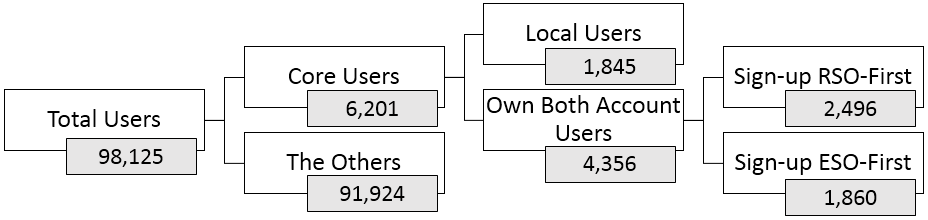
\includegraphics[width = 0.7\textwidth]{figures/usercomponent.png}
	\caption{User composition in Russian Stack Overflow}
	\centering
	\label{fig:usercomponent}
\end{figure}

If a core user in RSO who signs up ESO first and then RSO contributes comparatively less to ESO after signing up RSO, we say that RSO negatively influence this user's contribution to ESO.
To identify such users, we define the following formula: 

\begin{equation}
f = \frac{PostCountonESOAfterSignupRSO/DaysAfterSignupRSO}{PostCountonESOBeforeSignupRSO/DaysBeforeSignupRSO}	 
\label{equ:active}
\end{equation}

For a user who sign up ESO first and then RSO, this equation compares the user's average post number per day in ESO before and after the user signs up RSO.
The smaller value indicates that the user makes comparatively less contribution to ESO after signing up RSO.
%\textcolor{blue}{The smaller value represents the more possibility the user has migrated from Stack Overflow to Russian Stack Overflow. XINGZC: I think this formula alone tells only the posting behavior change on ESO after singing up RSO. Without contrasting it to the post behavior on RSO, i.e., average post per day on RSO, it cannot tell the migration from ESO to RSO. Maybe this users stop contributing to SO no matter ESO or RSO. Just like the stanislav example below, you need to study how many posts he contributes to RSO. Only if a user's contribution to RSO is comparable to his contribution to ESO before signing up RSO and his contribution to ESO decreases after signing up RSO, then we may guess this user migrate from ESO to RSO.}
%It means that if a core user in Russian Stack Overflow is more likely migrant if he creates fewer posts in Stack Overflow after his registration of the Russian one than that before his registration.
%\textcolor{red}{CCY to XINGZC:As all users analyzed here is core users, we assume they make big contributions to RSO. Once they contribute less in ESO after their RSO registration, we assume that they are migrating to ESO.}
Let's take one user as an example whose id is \textit{Vlad} in English Stack Overflow\footnote{\url{https://stackoverflow.com/users/276994}} and \textit{VladD} in the Russian one\footnote{\url{https://ru.stackoverflow.com/users/10105}}.  
He joined the ESO first on February 2010, and then joined the RSO on November 2012.
Before joining the RSO, he has answered 669 questions in ESO in about 2 years, but only answered 189 questions in ESO for 5 years after his join into RSO. 
Instead, he has answered 3,798 questions in RSO and earned 173,213 reputation score so far, while his current reputation score in ESO is only 28,781.
This user can be regarded as a user migrated from ESO to RSO.
%\textcolor{orange}{new example updated, whoes f value is around 0.37 but this user is a high reputation score users on both sites}

\begin{comment}
Moreover, for the 1,835 of Core Users who sign up the Stack Overflow account first,
according to their frequency of post activity, it can be also concluded that they are still
spending more time and concentrate on the Stack Overflow main site. The formula of
judging a migrant is Formula~\ref{equ:active}. If the f value is greater than 1, the user transferred his or her main active area to the new site.
\end{comment}


We consider $0.8 \leq f \leq 1.2$ as a reasonable range for relative stable level of contribution to ESO after the user signs up RSO.
That is, the user's posting behavior in ESO does not change significantly after signing up RSO if $0.8 \leq f \leq 1.2$.
%level that is 0.8 to 1.2 \textcolor{red}{1.2 ??why not 1?},since we consider that the user's active degree on English StackOverflow did not change significantly within this range.
%For $f$, the results in Table~\ref{tab:table3} reveal that more than half of those active users from the main site tend to be more active in a multilingual sub-site. Although they are from another site, they make a lot of contribution and seem to be like using the new sub-site regularly. 
%\textcolor{blue}{The following analysis needs to contrast $f$ with average post per day on RSO.}
%As seen in Table~\ref{tab:migrationCalculation}, 
Among 1860 core users in RSO who sign up ESO first, 120 (6.5\%) are with the $f$ value in range of 0.8 to 1.2, i.e., their contribution is relatively stable in ESO after signing up RSO.
1033 (55.5\%) users are even more active in ESO with $f>1.2$. 
Only 707 (38\%) users become less active in ESO.
It indicates that although many users from ESO contribute a lot to RSO, they do not stop making consistent contributions in ESO.
It further demonstrates that the launch of RSO will not cause severe community split of users between ESO and RSO. 
%The conclusion of the research on post aspect is the multilingual community has a group of users as backbone so that the community is not dominated by the users from the Stack Overflow main site, but the migrants from the main site are also willing to contribute in the new community.

\begin{comment}
\begin{table}
	\small
	\centering
	\caption{Posting Behavior Change for Core users Who Signs up ESO First then RSO \textcolor{blue}{I think we better not split the analysis by $>20, 50, 100$. For those $>50, 100$, most of f values decreases. This may means those most active users actually contribute relative less after signing up RSO. This is hard to explain.}}
	\label{tab:migrationCalculation}
	\begin{tabular}{lllll}
		\hline
		\textbf{\#RSO Post by User} & \textbf{\#User} & $\textbf{f < 0.8}$ & $\textbf{0.8<=f<=1.2}$ & $\textbf{f > 1.2}$ \\
		\hline
		$>=$10 & 1,860  &707 & 120 & 1033   \\
		$>=$20 & 445  & 208 & 39 & 198\\
		$>=$50 & 228 & 134 & 18 & 76 \\
		$>=$100& 134 & 94 & 11 & 29 \\
		\hline
	\end{tabular}
\end{table}		
\end{comment}

%\textbf{Summary:} The migrated users from Stack Overflow main site are not dominant in the Russian subsite.

\subsection{User Reputation Score}

%\textcolor{red}{
%I think we should have this reputation score analysis for those 6201 core users from the posting behavior analysis, rather than reputation score of users with an arbitrary reputation score cutoff 20. We should see how many local, users sign up ESO first, users sign up RSO first among these 6201 core users and then plot the R score of these 6201 core users in several intervals. 
%The current logic flow is awkward because we have two different ways to study users: active users with an arbitrary R score above 20, and core users who post more than 10. See also my comments below on the cutoff 20 and Fig.2.}
%\textcolor{blue}{CCY: 1) post number is not necessarily correlated to the reputation score as reputation score contains not only upvotes of posts, but also other post edits and tag wiki creation. So I want to see the power of ESO users in RSO from this aspect. 2)Yes, 20 is too arbitrary, have removed it.}
%\textcolor{red}{XINGZC: That is fine. But it may still be attacked.}
In Stack Overflow, users can earn reputation score if their questions, answers or comments get upvotes. 
They can also get bonus if they commit to editing others' posts, creating tag wiki which help to maintain the quality of the site.
So, apart from the number of posts, reputation score is another good indicator of how much contribution a user has made to the community and how much the community trusts his work.
%\textcolor{blue}{It has been used as a metric to identify active and credible users in the Q\&A sites~\cite{??findsomereferences,??,??} XINGZC: This may invite questions that why we do not use reputation score to identify users for posting behavior analysis?}.
%Figure~\ref{fig:reputationDistribution} shows the distribution of reputation score of 98,125 users in Russian Stack Overflow.
According to the privilege policy of Stack Overflow\footnote{\url{https://stackoverflow.com/help/privileges}}, users who earn more than 10 reputation score can remove the new user restriction. 
%To focus on the reputation distribution among the formal users, this section only includes 31,029 users with more than 10 reputation score on Russian Stack Overflow.}
As new users do not contribute much to the site, we only consider 31,029 users with more than 10 reputation score in RSO in this analysis.
These 31,029 users in RSO belong to three groups:
10,702 (34.5\%) local users who only register RSO,
12,292 (39.6\%) users who sign up ESO first and then sign up RSO,
and 8,035 (25.9\%) users who sign up RSO first and then sign up ESO.

\begin{figure}
	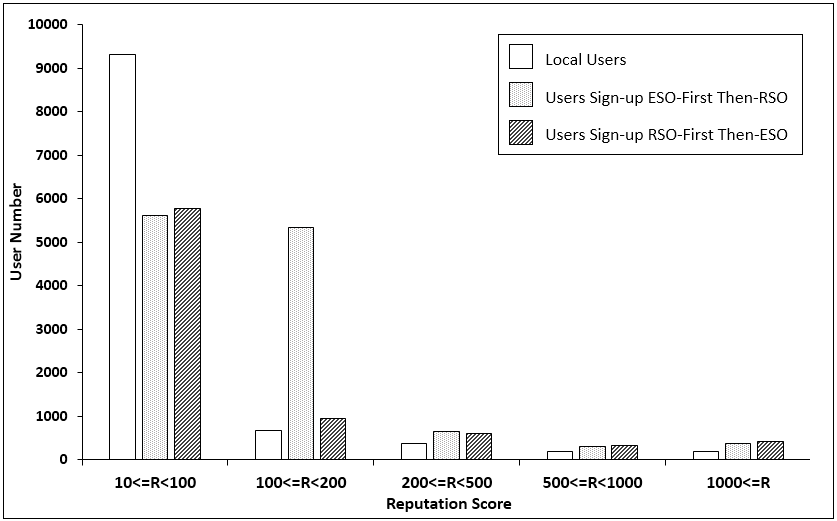
\includegraphics[width = 0.6\textwidth]{figures/reputation.png}
	\caption{The reputation distribution of three-group users in RSO}
	\label{fig:reputationDistribution}
\end{figure} 

Fig.~\ref{fig:reputationDistribution} shows the distribution of reputation score of these three groups of users in five different intervals.
We can see that the distributions of reputation score in the first two low-reputation intervals are different from those in the three high-reputation intervals.
This phenomenon is due to the Association Bonus Policy of Stack Exchange~\cite{web:associationBonus}.
According to this policy, a user will earn 100 bonus reputation score in RSO when the user signs up a RSO account, if the user has already owns an ESO account with 200+ reputation score.
Therefore, compared with local users and bi-account users who sign up RSO first, there is a relatively less proportion of bi-account users who sign up ESO first in the reputation interval $10 \leq R < 100$.
In contrast, a large proportion of bi-account users who sign up ESO first have reputation score within $100 \leq R \leq 200$.
This results in that the number of bi-account users who sign up ESO first is more than the sum of local users and bi-account users who sign up RSO first in the interval $100 \leq R \leq 200$.

But in the other three intervals (i.e., $R \geq 200$), we can see that the number of local users plus the number of users who sign up RSO first then ESO is more than the number of users who sign up ESO first.
%the number of users sign-up ESO-first then-RSO is roughly the same as the number of users sign-up RSO-first then-ESO
Furthermore, in the three intervals $R \geq 200$, there are roughly the same number of users in the group of users sign up ESO first and in the group of users sign up RSO first.
However, considering that there are 12,292 users in total who sign up ESO first and 8,035 users who sign up RSO first, the later group has much higher percentage of high-reputation users than the former group.

This analysis suggests that the community of RSO has its own core contributors.
However, its community is not completely independent of that of ESO, because a large number of users from ESO (especially high-reputation users from ESO) makes similar contribution to RSO, as those local users and those who sign up RSO first.	

\begin{comment}
Considering the Reputation Bonus Policy that a starting plus 100 reputation bonus 
to users who already have a 200+ account of any site belongs to Stack Exchange [5], the 32,288  users who migrated from the main site reasonably have a large number of 
the reputation level of 100 to 200. However, despite the local user, the remains are 
the user who owns both account of the main site and Russian version. Under the 
circumstance that the number of migrants is almost \textcolor{red}{2 times ??32288/19125 about 1.7 times, not 2. In a technical paper, has to be very specific} of that of the 19,125 users 
who sign up Russian version account first, \textcolor{red}{the later contributes somehow an equal 
number of active users ??how can we tell this from Fig. 3?}.

To some degree, the reputation reveals that multilingual communities \textcolor{red}{are not dominated 
by a large number of external users even the later has an overwhelming advantage 
on the user amount ??do not understand how this conclusion can be reached from the reputation distribution analysis?}, which means that multilingual communities are relatively 
independent in the respect of user contribution in the community development process.
\end{comment}


%In Stack Exchange, once a user get more than 200 reputation points, he will get site %association bonus i.e., 100 points on each site in Stack Exchange, as Stack Exchange regards %that user as trusted [5]
%~\cite{https://stackoverflow.com/help/whats-reputation}.
%Therefore, we regard users with 200+ reputation score in Russian Stack Overflow as its core %users.
%Considering the Reputation Bonus Policy that a starting plus 100 reputation bonus to users who already have a 200+ account of any site belongs to Stack Exchange [5], the 29,609 users who migrated from the main site reasonably have a large number of the reputation level of 100 to 200. 

%However, there are 384,304 core users in Stack Overflow, and only 885 of them migrate to %Russian Stack Overflow.
%Figure~\ref{fig:reputationDistribution} displays the detailed reputation score distribution, %and most migrated user actually lay in the range between 100 to 200.
%That is because the core user in Stack Overflow can get 100 reputation points once they join %Russian Stack Overflow, but they are not counted as active in the new site as they are not %active to get another 100 points.  
%Among 3,390 core users, only 885 (28.24\%) of them come from Stack Overflow.
%It demonstrates again that Stack Overflow is merely hurt by the launch of Russian Stack %Overflow, and Russian Stack Overflow is rather independent.
%However, despite the local user, the remains are the user who owns both account of the main site and Russian version. 


%\textcolor{red}{Actually, it is wrong to define migration as in this paper, because although some people come from Stack Overflow, they can only be regarded as migrated only if they are active in Russian Stack Overflow, but not active in the main site any more. But we do not have enough time to revise it.}

%\textbf{Summary:} 28.24\% core users in Russian Stack Overflow migrate from Stack Overflow.
%Under the circumstance that the number of migrants is almost 2 times of that of the 16,155 users who sign up Russian version account first, the later contributes somehow an equal number of active users.
%To some degree, the reputation reveals that multilingual communities are not dominated by a large number of external users even the later has an overwhelming advantage on the user amount, which means that multilingual communities are relatively independent in the respect of user contribution in the community development process.

\begin{comment}
Those are also people being targeted by the new site. So far for the argument that every decent programmer has to know English, some know it but just prefer their native language and I'd argue Matz is a more than decent programmer. As for most information being available in English and non-English information being bad, the first **public** release of ruby was in 1995 and by 2000 it was more popular than Python in Japan. The first English mailing list was created in 1999 but it took until 2002 for it to get as much messages as it's Japanese counter part (even though people from everywhere around the world could use it instead of just Japanese people). It actually took until Ruby 1.8 and 2003/2004 to get good documentation and books in English. That said we now got decent information about it in English available but there's also a massive Japanese community with wealth of information still, as one example Matz's own blog.	
\end{comment}

\vspace{2mm}
\noindent \fbox{\centering%
	\parbox{0.98\textwidth}{%
	   \textbf{Summary}: In term of post contribution and reputation score, Russian Stack Overflow benefits a lot from English Stack Overflow as many users in RSO come from ESO, especially those who can speak Russian.	
	   But there is no significant community split between the two sites, as those from-ESO users only account for a very small proportion of the user base in ESO and the majority of them still make stable contributions to ESO even after they sign up RSO.
	   In addition, RSO also helps to attract new users to ESO.    
	}%
}
\\
